\chapter{Doubling the evidence: Addition of twin studies}
\label{chap:seven}

So far, I have explored the role of schooling and its contribution to an individual's future earnings. Furthermore, I tried to answer the question of what role ability plays in this equation and whether or not it should be accounted for.
Even though I claim that some magnitude of ability bias exists in the relationship, one crucial question remains unanswered. This question is - to what extent is the increase in earnings influenced by schooling and to what extent by ability? Is there a way to separate these two and isolate the effect schooling has on an individual's wage, regardless of their ability? As it turns out, there is. Using a sample of twins, one may theoretically rule out the role of ability and family background and observe the unbiased influence of education on earnings. In the following chapter, I attempt to take this approach by constructing an entirely new dataset containing only natural twin studies. With this dataset, I will run the analysis anew and try to determine whether individual differences and innate ability play a crucial role in determining one's future or whether it is all just a matter of education.


\section{Understanding natural experiments: Is it all intertwined?}
\label{sec:twins_literature}

For this analysis, it is vital to understand how being a twin plays a significant role in the matter. We can identify two types of twins - monozygotic and dizygotic. Monozygotic twins (marked further as MZ twins), sometimes called identical twins, come from a single zygote and thus share the same genetic information. For this, it is reasonable to assume they share the same innate ability, and any noteworthy differences that arise during their lifetime should come from their environment, schooling, family background, etc. Dizygotic twins (marked further as DZ twins), on the other hand, come from two different zygotes, and their genetic information thus differs slightly. As such, these may be looked at more as siblings of the same age. For our purposes, monozygotic twins are of particular interest, as they allow us to isolate the role of innate ability from the equation.

Now let us take a look at the existing literature on the topic. Like twins sharing the same family background and living environment, the existing studies also share many similarities. The two studies of \cite{ashenfelter1994estimates} and \cite{ashenfelter1998income} perhaps stand as the cornerstones behind the current form and direction of the literature. In these studies, the authors construct a survey and study samples of twins to find that the \ac{OLS} estimate of returns to schooling is upward biased. In \cite{ashenfelter1994estimates}, the authors propose a new approach where the measurements of education are collected from both twins, and the final estimate comes from the within-twin comparison. This involves taking one twin's report of the within-twin schooling as an instrument for the other twin's report. The benefit of this approach lies in addressing the possible measurement error that sometimes arises in schooling reports. Several other studies, including \cite{behrman1994endowments}, \cite{isacsson1999estimates}, or \cite{bonjour2003returns}, too follow a similar approach and provide a solid theoretical background to the matter.

Another vital issue, as well as a critique of the twin approach, lies in the idea that the within-twin schooling differences may not be random but endogenous with respect to wages. \cite{bound1999double}, for example, argue that ability can be influenced by factors other than genes and that using methods such as \ac{IV} regression to remedy the measurement error can simultaneously increase the omitted ability bias. On the other hand, using techniques such as Fixed-effects estimator may remove the omitted variable bias but does so at the cost of introducing even greater bias in measurement error \citep{ning2005economic}.


% TODO - determine from Ning accurately how ability bias is measured, lie down the techniques, what they accomplish, and how can the results be calculated. Then consider whether to run the analysis on identical twins only (likely), then gather results.

% Without going into too much detail, the current literature leverages mostly six techniques. These are \ac{OLS}, \ac{GLS}, \ac{IV} regression, Fixed-effect estimator, First-differences, and First-differences by \ac{IV}. Given that the potential ability bias arises from the omission of the ability variable from the equation, techniques that treat omitted variable bias will help us identify the extent of the bias. Methods such as \ac{GLS} or \ac{IV} will help us accomplish precisely that. On the other hand, the Fixed-effect estimator, First-differences, and First-differences by \ac{IV}, all do a great job in eliminating the measurement error, but do not control for the ability bias. As a result, I expect these techniques to yield 

% . The other three methods, \ac{OLS}, \ac{GLS}, and \ac{IV} regression, do not account for the omitted ability bias and should, in theory, yield higher estimates of the returns to schooling. The flipside of this assumption is that it does not account for the measurement error. 

% While the first three are more likely to be plagued by the omitted ability bias, the latter three do consider it and should consequently account for it.  % Sources???


% Since this thesis is primarily concerned with the role of ability, I opt to leave out the measurement error issue and focus solely on the omitted ability bias. 

% By comparison of these two approaches, it should be possible to determine whether the ability bias exists in the natural experiment data, and what is its extent.



\section{What do you mean there are two?: Making a twin dataset}
\label{sec:twins_data}

I will construct the new dataset, comprising natural experiments, with two analysis goals in mind. First, as described in the previous section, I will attempt to quantify the omitted variable bias, and second, I will want to compare the results with the conclusions obtained from the earlier chapters. As such, the form of the dataset will be nearly identical to the one described in \autoref{chap:three}, with slight modifications to accommodate the specific design of the included studies.

As for the studies themselves, I start with the literature review of \cite{nakamuro2012estimating} and \cite{li2012estimating}, and from there, perform snowballing to identify as many relevant studies on the topic as possible. Using this approach, I collected, in total, 16 studies. For their complete list, see \autoref{app:one}.  Given how intertwined the studies on the topic are, perhaps due to the relatively small scope of the topic, the choice of which papers to include was somewhat streamlined. Possibly, I may have missed several studies, but I am highly confident that this set should provide a highly representative sample of the literature.

After collecting the data from these 16 studies, it became apparent that some variables were unusable for this particular use case. Two variables, \textit{Sector: Public/Private}, \textit{Sector: Urban/Rural}, had no observations associated with them at all, while the variables \textit{Control: Experience squared}, \textit{Control: Occupation}, and \textit{Education: Primary/Secondary/...} had fewer than ten. As such, I removed all these variables from the dataset, together with the \textit{Ability} variable, for the approach to measuring ability bias is slightly different now, as explained in \autoref{sec:twins_literature}. For some variable groups, only some sub-categories had no data, such as \textit{Estimate: Sub-region/Continent}, \textit{Micro Data}, \textit{Region: Lat-America/Middle East and North Africa/South Asia/Saharan Africa}, \textit{Income: Low}, \textit{Instrument: Distance to school}, and finally, \textit{Control: Health}. On the other hand, I also added a handful of new variables, including:

\begin{itemize}
  \item \textit{White/Non-white} - Ratio of white subjects to non-white subjects.
  \item \textit{Married/Unmarried} - Ratio of married subjects to non-married subjects.
  \item \textit{Identical/Non-identical/No twins} - Ratio of subjects that are either identical (MZ) or non-identical (DZ) twins or are not twins at all.
  \item \textit{Method: Selection/FE} - =1 if the authors use  Selection-effects or Fixed-effects estimation.
  \item \textit{Method: IV First-differenced} - =1 if the authors use First-Differenced IV estimation.
  \item \textit{Instrument: Smoking} - =1 if the authors use smoking as an instrument in the regression.
\end{itemize}

For the list of all variables used in the analysis and their descriptive statistics, see \autoref{tab:twins_new_vars}. For the list of descriptions of the rest of the variables, see \autoref{tab:var}. The final form of the new dataset includes 293 observations across 16 studies and can be found in the online appendix.

For brevity's sake, I choose not to focus in depth during the analysis on differences between subsets of data, save for the type of method used. However, several statistics that characterize the new group of subjects might be helpful to highlight here just to get a better picture of how this new dataset differs from the old one. Firstly, two-thirds of the data consist of identical twins, roughly 26\% of non-identical twins, and less than 10\% of non-twin subjects. Among these, about 70\% are married, nearly the same amount are white, and over 82\% live in high-income countries. The subjects spent, on average, around 12.4 in school and 17.8 years working. For over 95\% of them, the schooling statistic is reported in years, as opposed to levels. Other statistics, including variable groups capturing data type, estimation method, publication characteristics, etc., can all be found in the aforementioned \autoref{tab:twins_new_vars}.

\begin{table}[!htbp]
  \centering
  \scriptsize
  \singlespace
  \caption{Variables of the twin dataset}
  \label{tab:twins_new_vars}
  \begin{tabular}
    {
      @{\hskip\tabcolsep\extracolsep}
      l
      *{3}{c}
      |
      l
        *{3}{c}
      @{}
    }
    \toprule
    Variable                                                                & Mean   & SD                                                           & Obs   & Variable                                                               & Mean   & SD    & Obs \\
    \midrule
    Effect                                                                  & 6.251  & 2.76                                                         & 293   & Income: High                                                           & 0.823  & 0.383 & 241 \\
    \multicolumn{3}{l}{\textit{\hspace{0.1cm}Estimate characteristics}}     &        & Income: Middle                                               & 0.177 & 0.383                                                                  & 52                   \\
    Standard Error                                                          & 1.126  & 1.036                                                        & 293   & Median Expenditure                                                     & 4.214  & 3.901 & 293 \\
    Estimate: City                                                          & 0.338  & 0.474                                                        & 99    & Minimum Wage                                                           & 3.025  & 2.761 & 293 \\
    Estimate: Region                                                        & 0.055  & 0.228                                                        & 16    & Acad. Freedom Index                                                    & 0.786  & 0.241 & 293 \\
    Estimate: Country                                                       & 0.608  & 0.489                                                        & 178   & Mean Age                                                               & 3.653  & 0.100 & 293 \\
    \multicolumn{3}{l}{\textit{\hspace{0.1cm}Data characteristics}}         &        & \multicolumn{3}{l}{\textit{\hspace{0.1cm}Estimation method}} &                                                                                                       \\
    Study Size                                                              & 3.000  & 0.426                                                        & 293   & Method: OLS                                                            & 0.345  & 0.476 & 101 \\
    Yrs. of Schooling                                                       & 12.463 & 1.456                                                        & 293   & Method: GLS                                                            & 0.102  & 0.304 & 30  \\
    Yrs. of Experience                                                      & 17.875 & 5.627                                                        & 293   & Method: Selection/FE                                                   & 0.253  & 0.435 & 74  \\
    Education: Years                                                        & 0.959  & 0.199                                                        & 281   & Method: FD                                                             & 0.034  & 0.182 & 10  \\
    Education: Levels                                                       & 0.041  & 0.199                                                        & 12    & Method: IV-FD                                                          & 0.068  & 0.253 & 20  \\
    Wage: Hourly                                                            & 0.287  & 0.453                                                        & 84    & Method: IV                                                             & 0.198  & 0.399 & 58  \\
    Wage: Daily                                                             & 0.130  & 0.337                                                        & 38    & Instr.: Sibling Ed.                                                    & 0.140  & 0.348 & 41  \\
    Wage: Monthly/Annual                                                    & 0.584  & 0.494                                                        & 171   & Instr.: Smoking                                                        & 0.061  & 0.241 & 18  \\
    Survey Data                                                             & 0.689  & 0.464                                                        & 202   & Instr.: Other                                                          & 0.048  & 0.214 & 14  \\
    National Register Data                                                  & 0.311  & 0.464                                                        & 91    & Control: Age                                                           & 0.584  & 0.494 & 171 \\
    Cross-sectional Data                                                    & 0.498  & 0.501                                                        & 146   & Control: Age$^2$                                                       & 0.478  & 0.5   & 140 \\
    Panel Data                                                              & 0.502  & 0.501                                                        & 147   & Control: Experience                                                    & 0.218  & 0.414 & 64  \\
    Data Year                                                               & 3.297  & 1.286                                                        & 293   & Control: Ethnicity                                                     & 0.157  & 0.364 & 46  \\
    \multicolumn{3}{l}{\textit{\hspace{0.1cm}Spatial/Structural variation}} &        & Control: Gender                                              & 0.522 & 0.5                                                                    & 153                  \\
    Wage Earners                                                            & 0.962  & 0.052                                                        & 102   & Control: Marriage                                                      & 0.416  & 0.494 & 122 \\
    Gender: Male                                                            & 0.557  & 0.277                                                        & 265   & Control: Firm Char.                                                    & 0.123  & 0.329 & 36  \\
    Gender: Female                                                          & 0.443  & 0.277                                                        & 28    & Control: Area                                                          & 0.055  & 0.228 & 16  \\
    White                                                                   & 0.694  & 0.421                                                        & 190   & Control: Macro Var.                                                    & 0.038  & 0.19  & 11  \\
    Ethnicity: Caucasian                                                    & 0.208  & 0.407                                                        & 61    & \multicolumn{3}{l}{\textit{\hspace{0.1cm}Publication characteristics}} &                      \\
    Married                                                                 & 0.699  & 0.143                                                        & 268   & Impact Factor                                                          & -0.269 & 1.125 & 206 \\
    Unmarried                                                               & 0.301  & 0.143                                                        & 252   & Citations                                                              & 3.855  & 2.173 & 293 \\
    Twins: Identical                                                        & 0.640  & 0.415                                                        & 242   & Study: Published                                                       & 0.703  & 0.458 & 206 \\
    Twins: Non-Identical                                                    & 0.263  & 0.377                                                        & 126   & Study: Unpublished                                                     & 0.297  & 0.458 & 87  \\
    Twins: None                                                             & 0.097  & 0.275                                                        & 34    & Publication Year                                                       & 1.018  & 0.898 & 264 \\
    \bottomrule
    \multicolumn{8}{>{\scriptsize}p{0.9\linewidth}}{\emph{Note:} This table presents basic summary statistics for variables of the new twin dataset. For detailed descriptions of all variables unmentioned in this chapter, see \autoref{tab:var}. SD = Standard Deviation, OLS = Ordinary Least Squares, GLS = Generalized Least Squares, FE = Fixed-Effects, IV = Instrumental Variable.}
  \end{tabular}
\end{table}


\section{Empirical analysis: Are the results just identical?}
\label{sec:twins_analysis}

As far as the outcome of the analysis is concerned, I will focus only on a handful of easily presentable results to keep the chapter concise.  The first is the publication bias issue, which can be summarized in a single table and should not be omitted even from this analysis. In \autoref{tab:PB-Twins}, I present the results of all linear, non-linear, and endogeneity-robust tests and methods explained in \autoref{chap:four}. That is, all but one, as there were too many non-linear techniques to fit into the table nicely; I decided to remove the Hierarchical Bayes results arbitrarily. For clarity, I add that the test for publication bias using said method yielded a coefficient of 0.60 with a standard error of 0.36. In contrast, the coefficient associated with the effect was estimated at 6.85 with a standard error of 0.54 over 293 observations. The rest of the results can be found in the table mentioned above.

% Linear tests
\afterpage{
  \begin{table}[!htbp]
    \centering
    \small
    \singlespace
    \caption{Twin studies are plagued by publication bias}
    \label{tab:PB-Twins}
    \begin{tabular}{
        @{\hskip\tabcolsep\extracolsep}
        l*{5}{c}} %one left column, five center (*{} makes the cols inherit attributes)
      \toprule
      \multicolumn{6}{l}{\textit{Panel A: Linear methods}}                                            \\
      \multicolumn{1}{c}{}                  &
      \textbf{OLS}                          &
      \textbf{FE}                           &
      \textbf{RE}                           &
      \textbf{Study}                        &
      \textbf{Precision}                                                                              \\
      \midrule

      Publication bias                      & 1.347*** & 0.602*** & 0.840*** & 0.947*** & 2.897***    \\
      \emph{\hspace{0.2cm}(Standard error)} & (0.138)  & (0.162)  & (0.154)  & (0.177)  & (0.442)     \\
      \addlinespace[0.5em]
      Effect beyond bias                    & 4.735*** & 5.574*** & 5.55***  & 4.754*** & 3.907***    \\
      \emph{\hspace{0.2cm}(Constant)}       & (0.175)  & (0.219)  & (0.342)  & (0.185)  & (0.232)     \\
      \addlinespace[0.5em]
      Observations                          & 293      & 293      & 293      & 293      & 293         \\

      \midrule

      \multicolumn{6}{l}{\textit{Panel B: Non-linear methods}}                                        \\
                                            &
      \textbf{WAAP}                         &
      \textbf{Top10}                        &
      \textbf{Stem}                         &
      \textbf{AK}                           &
      \textbf{Kink}                                                                                   \\
      \midrule
      Publication bias                      &          &          &          & 2.257*** & 2.895***    \\
                                            &          &          &          & (0.126)  & (0.435)     \\
      \addlinespace[0.5em]
      Effect beyond bias                    & 5.77***  & 4.314*** & 3.403*** & 5.616*** & 3.908***    \\
                                            & (0.159)  & (0.265)  & (0.95)   & (0.157)  & (0.093)     \\
      \addlinespace[0.5em]
      Observations                          & 293      & 293      & 293      & 293      & 293         \\

      \midrule

      \multicolumn{6}{l}{\textit{Panel C: Methods relaxing the exogeneity assumption}}                \\
      \multicolumn{4}{c}{}                  &
      \textbf{IV}                           &
      \textbf{p-uniform*}                                                                             \\
      \midrule
      Publication bias                      &          &          &          & 1.824*** & L = 1.712   \\
                                            &          &          &          & (0.159)  & (p = 0.191) \\
      \addlinespace[0.5em]
      Effect beyond bias                    &          &          &          & 4.198*** & 7.79        \\
                                            &          &          &          & (0.188)  & (NA)        \\
      \addlinespace[0.5em]
      Observations                          &          &          &          & 293      & 293         \\

      \bottomrule
      \multicolumn{6}{>{\footnotesize}p{0.95\linewidth}}{\emph{Note:} Panel A: Results obtained from estimating the linear equation \autoref{eq:fat_reg}. Standard errors, clustered at the study level, are included in parentheses. OLS = Ordinary Least Squares. FE = Fixed Effects. RE = Random Effects. Precision = Estimates are weighted by the inverse of their standard error. Study = Estimates are weighted by the inverse number of observations reported per study. Panel B: Estimates of the effect and publication bias using five non-linear methods. WAAP = Weighted Average of the Adequately Powered \citep{Ioannidis2017Waap}, Top10 = Top10 method by \cite{Stanley2010Top}, Stem = the stem-based method by \cite{Furukawa2019Stem} where P represents the probability of results insignificant at 5\% are published relative to the probability of the significant ones at the same level, AK = \cite{Andrews2019Selection}'s Selection model, Kink = Endogenous kink model by \cite{Bom2019Kink}. Standard errors, clustered at the study level, are included in parentheses. Panel C: Estimates of the effect and publication bias using two techniques that relax the exogeneity assumption. IV = Instrumental Variable Regression; the inverse of the square root of the number of observations is used as an instrument for the standard error. Standard errors, reported in parentheses, are also clustered at the study level. P-uniform* = method proposed by \cite{vanAert2021puni}; L represents the publication bias test t-statistic, the corresponding p-value can be found in parentheses. ***p<0.01, **p<0.05, *p<0.1}
    \end{tabular}
  \end{table}
  \clearpage
}

A clear takeaway from these tests, which also holds across different methods and approaches, is that publication bias is considerably more prominent in the twin dataset than in the primary dataset, as explored in \autoref{chap:four}. With 6.2\% from \autoref{tab:twins_new_vars} as the baseline, the returns to schooling drop by an average of two, sometimes up to three percentage points. Namely, the STEM-based method suggests returns to education of 3.4\%, while the Endogenous Kink approach claims 3.9\%. On the other end of the spectrum, \ac{WAAP} and the Selection model report the highest returns, 5.7\%, and 5.6\%, respectively. No method reports a coefficient of schooling higher than the simple data average, save for p-uniform*, where the standard error failed to be estimated.

Moving on from publication bias, the crux of the matter, which I would like to focus on in terms of analysis outcomes, is the influence of different methods. As outlined in \autoref{sec:twins_literature}, the difference in approach to the omitted ability bias could have us conclude that if the results of the six employed methods vary only a little, the ability bias in the twin studies is not present. On the other hand, if they vary greatly, meaning the estimates of methods controlling for ability are lower than their counterparts, then that would suggest evidence to the contrary.

As a first insight into the influence of different methods on the outcome, I present both numerically and graphically how the returns to education effects behave when employing each of the six methods. In \autoref{fig:twins_prima_facie}, densities of the effect are displayed under different method specifications, while descriptive statistics of the effect behavior under said specifications can be found in \autoref{tab:twins_sum_stats}.

% Include means for subsets of data
\begin{table}[!t]
  \centering
  \scriptsize
  \singlespace
  \caption{Summary statistics for the twin dataset using different estimation methods}
  \label{tab:twins_sum_stats}
  \begin{tabular}{
    @{}
    l % Description
    *{6}{c} % Middle columns
    >{\centering\arraybackslash}p{1cm} % Last column with fixed width
    @{}
    }
    \toprule
                                 & \multicolumn{3}{c}{Unweighted} & \multicolumn{3}{c}{Weighted}        &                                                                      \\
    \cmidrule(lr){2-4} \cmidrule(lr){5-7}
                                 & Mean                           & \multicolumn{2}{c}{95\% conf. int.} & Mean   & \multicolumn{2}{c}{95\% conf. int.} & N. obs                \\

    \midrule


    \multicolumn{8}{l}{\textit{Baseline methods}}                                                                                                                              \\
    Method: OLS                  & 5.686                          & 1.648                               & 9.724  & 5.754                               & 1.716  & 9.792  & 101 \\
    Method: GLS                  & 7.363                          & 1.822                               & 12.904 & 8.005                               & 2.464  & 13.546 & 30  \\
    Method: IV                   & 7.155                          & 1.644                               & 12.666 & 7.570                               & 2.059  & 13.081 & 58  \\
    \midrule
    \multicolumn{8}{l}{\textit{Methods that treat the omitted ability bias}}                                                                                                   \\
    Method: Selection/FE         & 4.917                          & 0.515                               & 9.319  & 5.630                               & 1.228  & 10.032 & 74  \\
    Method: First Differences    & 7.920                          & 3.979                               & 11.861 & 7.916                               & 3.975  & 11.857 & 10  \\
    Method: IV First-Differenced & 8.689                          & 1.035                               & 16.343 & 8.725                               & 1.071  & 16.379 & 20  \\

    \bottomrule

    \multicolumn{8}{>{\scriptsize}p{0.85\linewidth}}{\emph{Note:} This table presents basic summary statistics of the returns to an additional year of schooling coefficient calculated on various subsets of the data. Unweighted = Original dataset is used. Weighted = Estimates are weighted by the inverse number of estimates reported by each study. OLS = Ordinary Least Squares, GLS = Generalised Least Squares, IV = Instrumental Variable, FE = Fixed-Effects. For cutoff points, medians are used except for dummy variables, where the cutoffs are 0.5.}
  \end{tabular}
\end{table}

No obvious pattern appears between the two groups of methods, that is, between the group that does treat the omitted ability bias and the one that does not. While estimates reported by \ac{OLS} and the Selection/Fixed-Effects methods suggest the lowest estimates of all (5.6\% and 4.9\%, respectively), when observing the difference in their estimates as per \cite{li2012estimating}, it comes up to only around 0.7\% (5.6 - 4.9). Even when looking at the weighted average of estimates for these methods, the discrepancies are overall minimal. On balance, this simple glance into the data suggests that treating the ability during the estimation of twin data samples presents only a marginal effect.



% Twins prima facie
\clearpage
\begin{figure}[!htbp]
  \begin{center}
    \caption{Returns to education for twins vary based on the method}
    \label{fig:twins_prima_facie}
    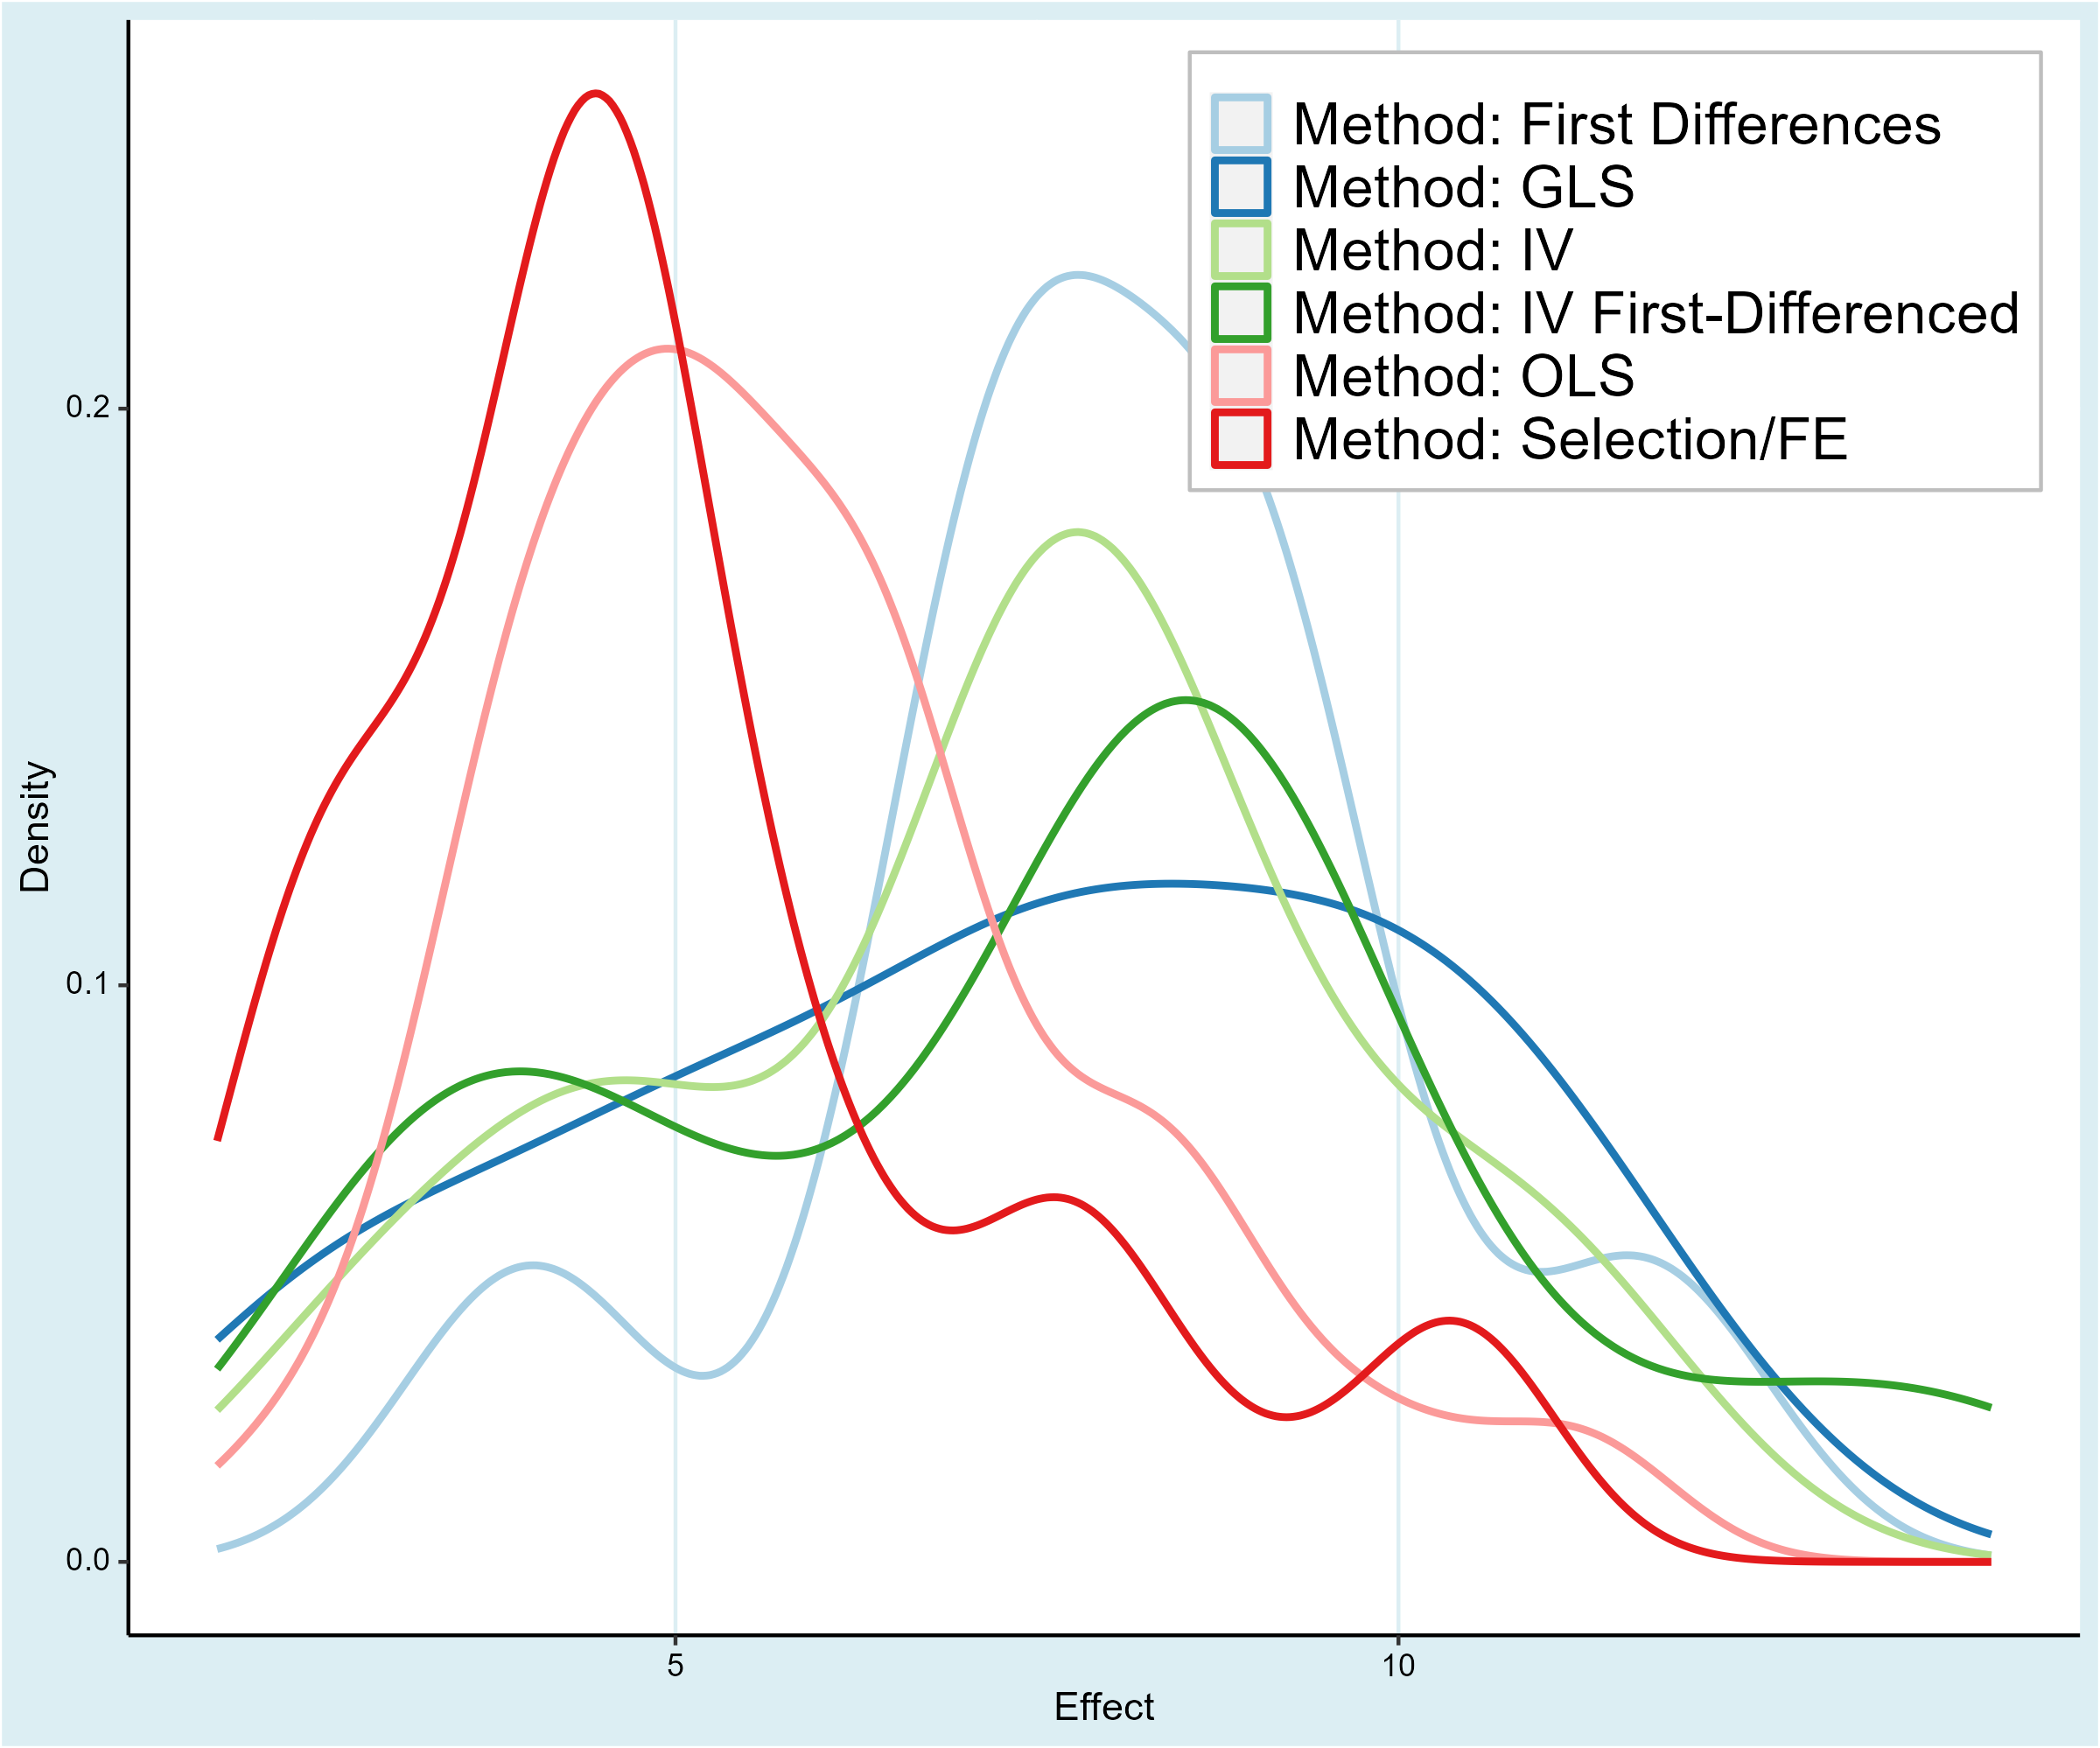
\includegraphics[width=0.9\textwidth]{Figures/twins_prima_method.png}
  \end{center}\vspace{-0.7cm}
  \captionsetup{width=0.9\textwidth, font = scriptsize}
  \caption*{\emph{Note:} This figure displays the densities of the effect of returns to education for twins under different method specifications. The effect is plotted on the x-axis against its density on the y-axis. For a description of the variables used in these figures, refer to \autoref{sec:twins_data}.}
\end{figure}




% Focus on the BMA coefficients for the methods too

% Include a FAT table of fat-pet tests, all on one page, cause no explanations needed - perhaps put in the appendix, dunno

% BPE results and graphs are in order I guess, as are the BMA results


%%%%%%%%%%%%%%%%%%%%%%%%%%%%%%%%%%%%%%%%%%%%%%%%%%%%%%%%%%%%%%%%

%% Notes on theory for self

%Check Li et al. (2012) Appendix Table A1 for concrete figures of ability bias $\to$ omitted variable bias (ability bias) = OLS - FE

%-BMA $\to$ - pub year causing problems, also 10 groups removed using automatic BMA

%Ning (2005) says -> "The
%Fixed-Effect estimator eliminates the omitted variable bias but it does so at the expense of introducing far greater measurement error bias."

%Further, measurement error.
%"A straightforward consistent estimator for equations (6) and (7) or (4) may be obtained by the method of instrumental variables using the independent measure of the schooling variables as instruments". In other words, if the reported schooling is instrumented with the other twins' reported schooling, the measurement error should disappear!!

% Cool twin theory in Bingley et al. (2005)
% A second approach uses within-twins differences in wages and education, assuming that unobserved effects (such as abilities, tastes, motivations, and preferences) are common within twins. However, studies based on siblings or twins have been criticized for two primary reasons. First, if ability consists of both an individual component as well as a family component, which is endogenous to the schooling variable, the within-family approach may not result in estimates that are less biased than OLS estimates. Second, if there is measurement error in the schooling variable, this will account for a large portion of the differences between the twins than across the population as a whole (Ashenfelter et al., 2000).
% KENAYATHULLA, Husaina Banu. "Higher levels of education for higher private returns: New evidence from Malaysia." International Journal of Educational Development, 2013, 33.4: 380-393.